%
% anwendungen.tex -- Anwendungen des Reed-Solomon-Codes
%
% (c) 2021 Michael Steiner, Hochschule Rapperswil
%
\section{Anwendungen des Reed-Solomon-Codes
	\label{reedsolomon:section:anwendung}}
\rhead{Anwendungen}

In den vorherigen Abschnitten haben wir betrachtet, wie Reed-Solomon-Codes in der Theorie funktionieren. 
In diesem Abschnitt werden wir einige Anwendungen vorstellen, bei denen ein Reed-Solomon-Code zum Einsatz kommt.

All diese Anwendungen teilen das gleiche Problem: Die Daten können nur durch einen höchstwahrscheinlich fehlerbehafteten Kanal empfangen werden. Es gibt keine andere Methode, an diese Daten zu kommen, als über diesen Kanal.

In der Netzwerktechnik zum Beispiel ist es üblich, dass bei Paketverluste oder beschädigt empfangene Datenpaketen diese einfach noch einmal innert wenigen Millisekunden angefordert werden können.
\index{Paketverluste}%
In der Raumfahrt ist dies nicht möglich, da aufgrund der beschränkten Speichermöglichkeit die gesammelten Daten so rasch wie möglich zur Erde gesendet werden. 
\index{Raumfahrt}%
Diese Daten wiederum brauchen aufgrund der grossen Distanz Stunden bis die Daten beim Empfänger ankommen.
Fehlerhafte Daten können also auf Grund der Zeitverzögerung nicht mehr angefordert werden. 

Bei CDs oder DVDs gibt es zwar kein zeitliches Problem, jedoch erschweren Kratzer, Verschmutzungen oder Produktionsfehler das Lesen einer solchen Disk.
\index{CD}%
\index{Compact-Disc}%
\index{DVD}%
\index{Digital Video Disk}%
Da vor allem Produktionsfehler und Kratzer irreversibel sind und die Disk nicht nach jedem Kratzer ersetzt werden, wird die korrekte Ausgabe der gespeicherten Information durch die Fehlerkorrektur sichergestellt. 

Einen ähnlichen Ansatz verfolgen QR-Codes, wobei die Information auch dann noch gelesen werden kann wenn der Code nicht mehr vollständig vorhanden ist. 
\index{QR-Code}%

%Wie man sieht, eignen sich Reed-Solomon-Codes vor allem für Anwendungen, bei der die Informationen nicht auf einen Anderen Weg beschafft werden kann. 
%
%
%, bei denen die Wahrscheinlichkeit hoch ist, dass während der Übertragung 
%
%Es ist deshalb umso wichtiger die Daten codiert zu lesen um so gleich die Lesefehler zu korrigieren.
%
% da aufgrund der grossen Distanz Stunden vergehen können bis gesendete Daten auf der Erde empfangen werden kann. 
%

Obwohl alle diese Codes nach dem gleichen Prinzip arbeiten gibt es starke Unterschiede in deren Funktionsweise. 
Dies kommt vor allem daher, da die Codes nur Ressourcen zur Verfügung haben, die von der Hardware bereitstellt wird,  auf denen die Codes implementiert wurden.
Diese Codes bedienen sich daher verschiedener Tricks und Optimierungen um möglichst effizient zu arbeiten.

Um die Fähigkeit eines verwendeten Reed-Solomon-Codes zu beschreiben verwendet man die Notation ($n$,$k$), wobei $n$ die Grösse des Nachrichtenblocks angibt und $k$ die Anzahl der Stellen, die für Nutzdaten gebraucht werden können.

%Dies kommt vor allem daher, da diese Codes an ihre Hardware gebunden sind, auf denen sie implementiert worden sind.
%Deshalb wurden diese Codes stark optimiert damit sie möglichst Effizient arbeiten können. 
%
%Um diese Hardware möglichst effizient zu nutzen wurden gewisse mathematische tricks angewendet um den Code möglichst effizient zu nutzen. 
%
% um mit maximaler Effizienz zu arbeiten. 
%Es überrascht daher nicht, dass vor allem ältere Codes im binären Körper $\mathbb{F}_{2}$ arbeiten.
%
% um den Code mit maximaler Effizienz zu nutzen. 
%
%Alle diese Anwendungen verfügen über eigene spezifizierten Eigenschaften.
%
%, wobei bei allen dieser Anwendungen jeweils eine unterschiedliche Version des Codes implementiert wurden.
%
%Dies kommt vor allem daher, da diese Codes immer an ihre dementsprechende Hardware gebunden sind, auf denen sie implementiert wurden um den Code mit maximaler Effizienz zu nutzen. 
%
% eigene Version des Codes implementiert haben. 
%
%Bei einer Technischen Umsetzung eines solchen Codes werden wir auf eine reihe neuer Probleme stossen wie Ressourceneffizienz, Laufzeitoptimierung, usw.
%
%Hinzu kommt, dass für verschiedene Anwendungen verschiedene Versionen des Reed-Solomon-Codes zur Anwendung kommen.
%
%Nachfolgend werden wir ein paar dieser Anwendungen Vorstellen, da sich herausstellt, dass Reed-Solomon-Code sehr 
%
%Als letzte Frage stellt sich jetzt nur noch, wo diese Codes eingesetzt werden. 
%
%Bisher haben wir 
%
%In den letzten abschnitten haben wir uns ausführlich die Funktionsweise des Reed-Solomon-Codes angeschaut. In diesem Abschnitt möchten wir dem Leser ein paar bekannte beispiele vorstellen, in denen Reed-Solomon-Codes zum einsatz kommen. Es sei jedoch angemerkt, dass diese Anwendungen in der Umsetzung oft ein wenig anderst funktionieren als hier vorgestellt. Dies wurde vor allem wegen technischen optimierungen realisiert. (technische tricks und finessen), von der logik jedoch sehr stark an unserem Beispiel orientieren

\begin{figure}
	\centering
	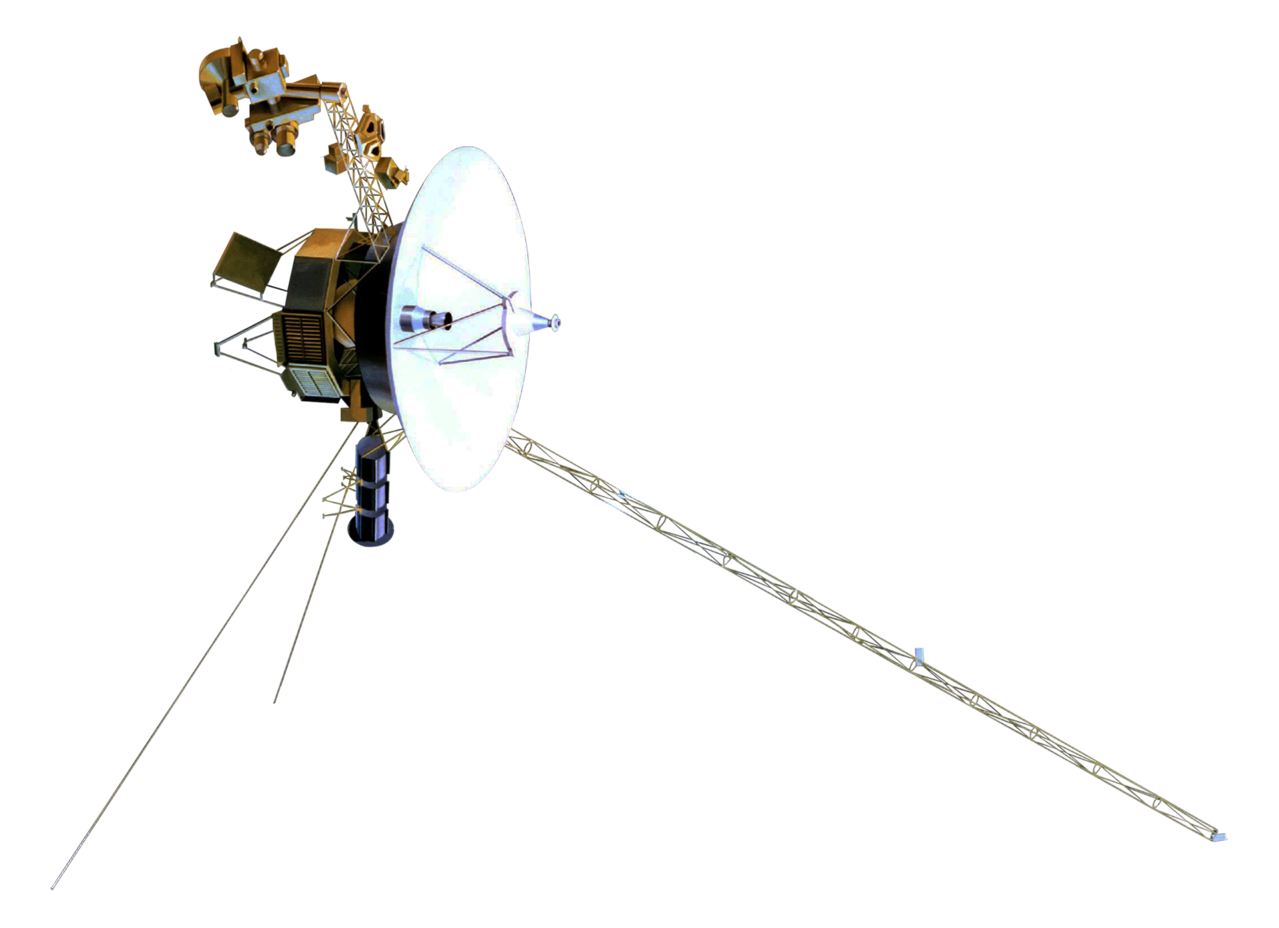
\includegraphics[width=0.5\textwidth]{papers/reedsolomon/images/Voyager_Sonde}
	\caption{Mit einer Entfernung von über 22.8 Milliarden Kilometer ist die Voyager 1 Raumsonde das am weitesten entfernte, von Menschen erschaffene Objekt. Obwohl ihre Schwestersonde Voyager 2 zuerst ins All gestartet wurde befindet Sie sich ``nur'' 19 Milliarden Kilometer weit weg von der Erde. Aufgrund abnehmender Batterieleistung werden die beiden Sonden ihre wissenschaftlichen Aktivitäten etwa 2025 einstellen, bleiben aber bis in die 2030er mit uns in Kontakt.}
\index{Voyager 1 und 2}%
	\label{fig:voyager}
\end{figure}

\subsection{Raumfahrt}
Obwohl Reed-Solomon-Codes bereits in den 1960er entwickelt wurden fanden sie erstmals Anwendung in der Voyager Raumsonde der NASA. Die Daten der zwei im Jahre 1977 gestarteten Sonden (siehe Abbildung \ref{fig:voyager}) werden mit einem ($255$,$233$)-Code
\index{Voyager Raumsonde}%
\index{NASA}%
codiert. 
Der Nachrichtenblock hat somit eine Länge von $255$ Zahlen, wovon $233$ als Nutzlast zur Verfügung stehen.
Damit ist es möglich bis zu $11$ Fehler im Nachrichtenblock zu korrigieren. 
Der codierte Nachrichtenblock wird in kleinere Blöcke aufgeteilt, mit einem Faltungscode erneut codiert und anschliessend gesendet.
Ein Faltungscode ist wie ein Reed-Solomon-Code in der Lage Fehler zu korrigieren, 
codiert seine Information aber auf eine andere Weise. Aus jedem unterteilten Block wird vor dem Versenden ein Paritätsbit erzeugt und dem Block angehängt. Anhand dieses Paritätsbits überprüft der Empfänger, ob bei der Übertragung der Block beschädigt wurde. Ist dies der Fall, wird der Block bei der Decodierung nicht beachtet. Diese so entstandenen ``Lücken'' im Datenstrom werden wiederum vom Reed-Solomon-Code korrigiert. Dieses Zusammenspiel beider Codes garantiert so eine hohe Robustheit gegenüber Übertragungsfehler. 

\begin{figure}
	\centering
	\subfigure[]{
	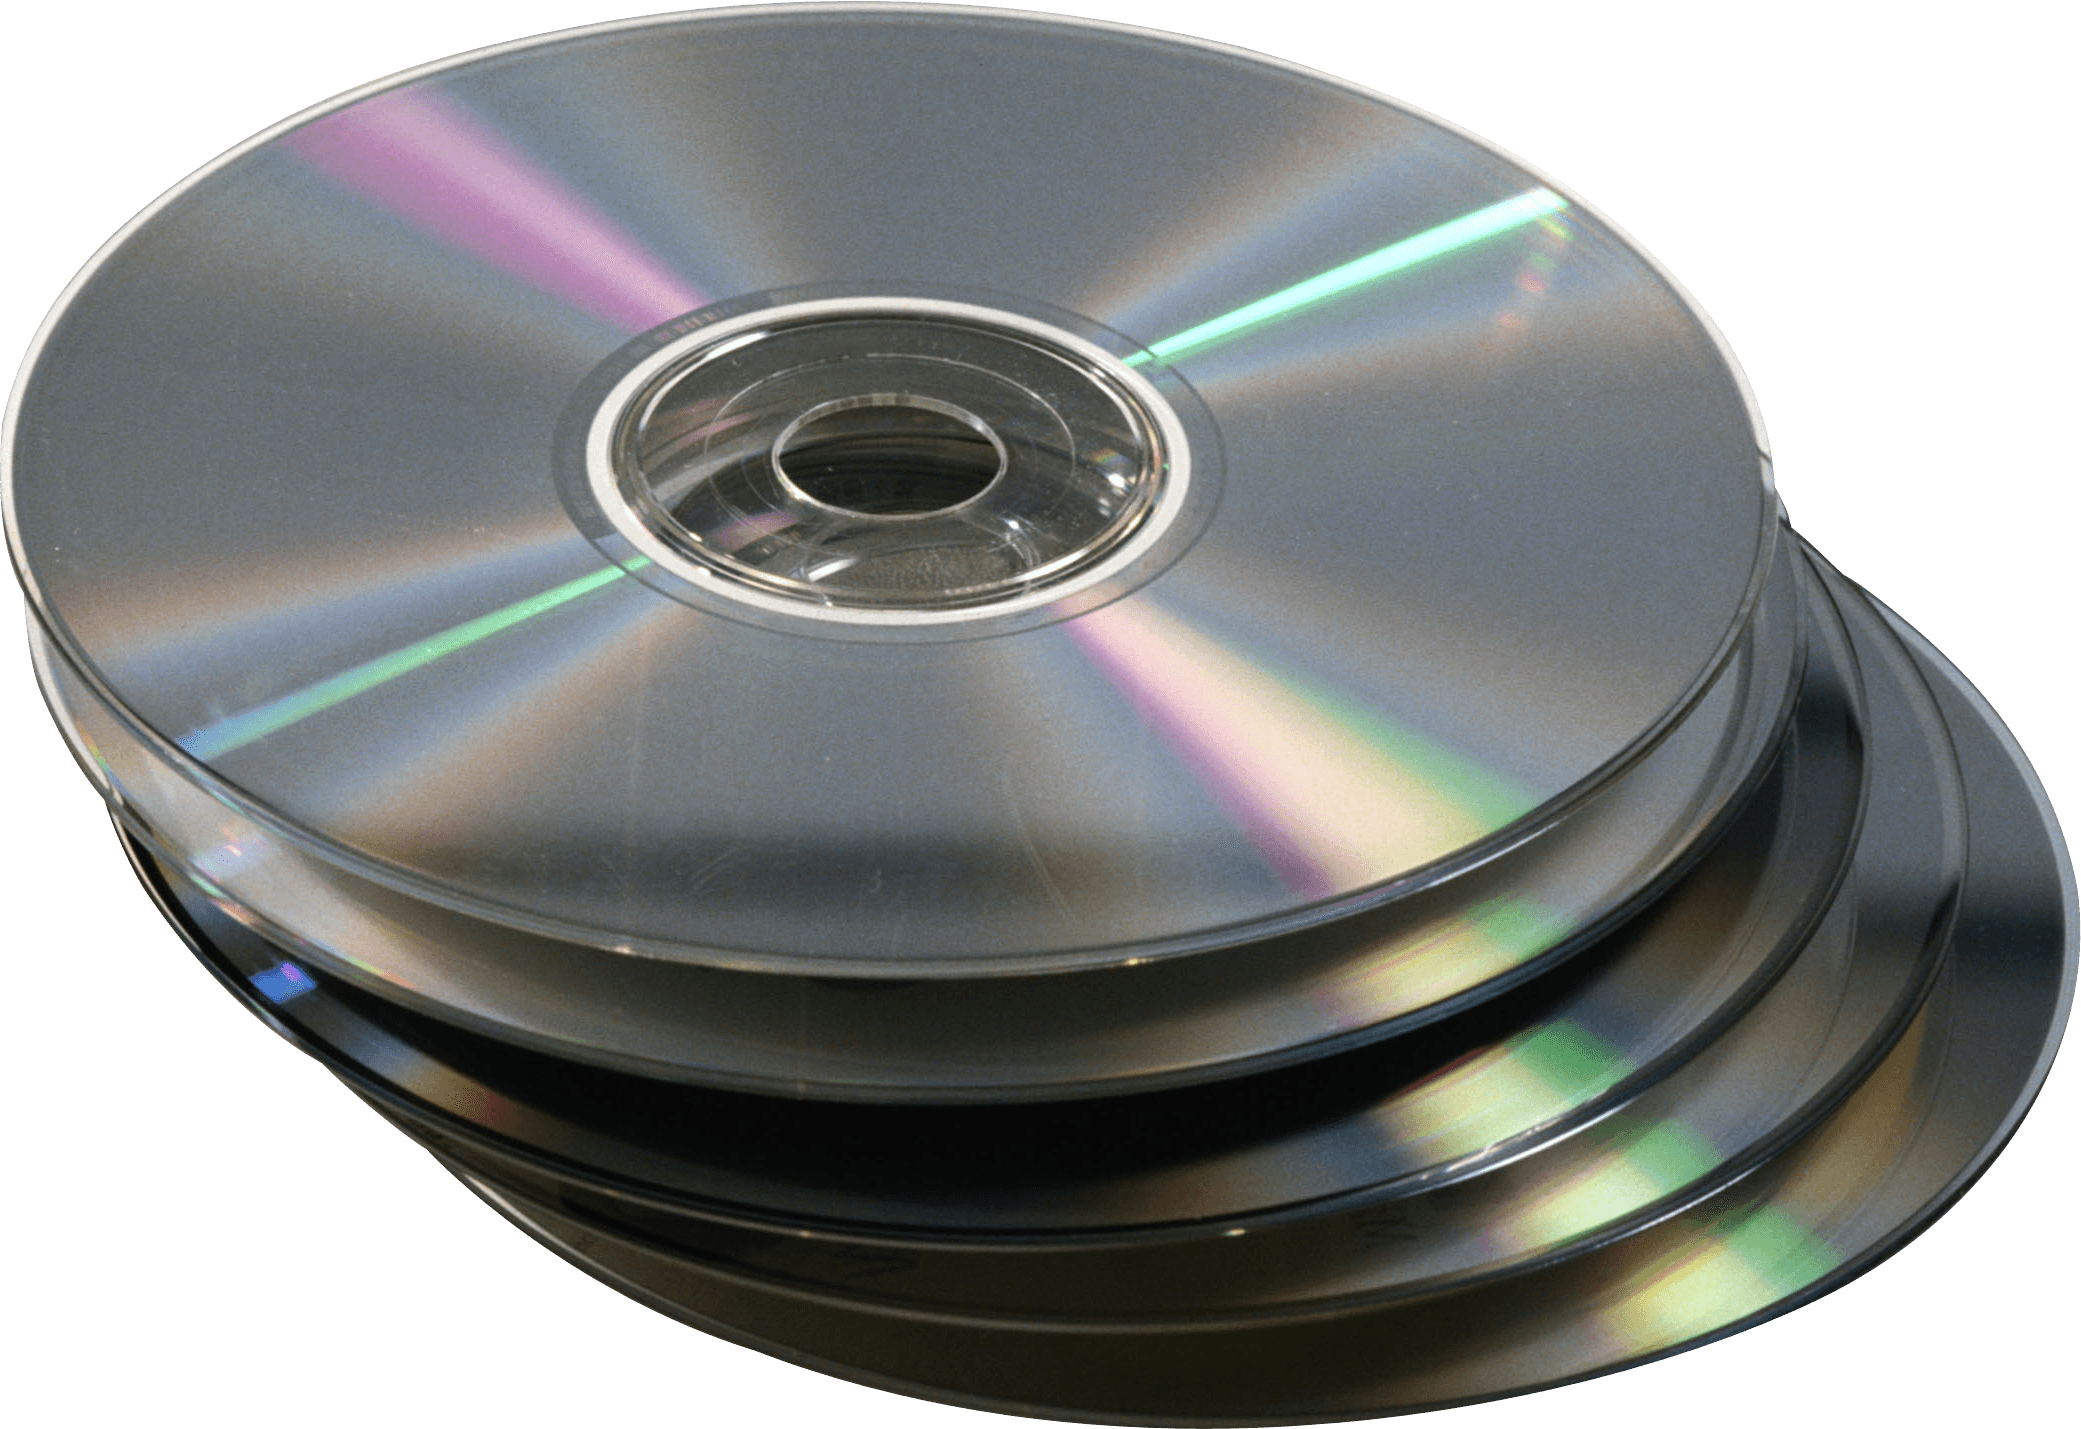
\includegraphics[width=0.45\textwidth]{papers/reedsolomon/images/Compact_Disc}
	}
	\subfigure[]{
		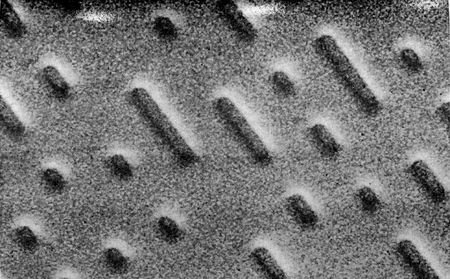
\includegraphics[width=0.45\textwidth]{papers/reedsolomon/images/Compact_Disc_zoomed_in}
	}
	\caption{CDs kamen 1982 auf den Markt. Sie funktioniert durch das Einpressen oder Einbrennen von Punkten und Strichen, die die Daten repräsentieren. Gelesen werden diese wiederum durch die Reflektion eines Lasers an diesen Punkten und Strichen.}
	\label{fig:cd}
\end{figure}
% 
% Funktioniert aber nach einem ganz anderen Prinzip. 
%
%Durch diese doppelte Codierung wird eine äusserst hohe Übertragungssicherheit garantiert.
%
%Dabei steht die Zahl 255 für grösse des Nachrichtenblocks, der die Anzahl 233
%
%
% \textcolor{red}{benötigt das weitere Erklärungen, wie z.b. 255: grösse Nachrichtenblock, 233: anzahl der nutzbaren daten ?} zusammen mit einem konventionellen Faltungscode übertragen. Eine von der Sonde gesendete Nachricht hat eine Blockgrösse von 255 Zeichen, wovon 233 für die Nutzdaten gebraucht werden können. Dieser Code ist somit in der Lage 11 Fehler in einem Nachrichtenblock zu korrigieren. 
%
% Die zwei im Jahre 1977 gestarteten Sonden senden Daten mit der Hilfe eines RS(255,233)-Code für die digitalen Bilder sowie einem konventionellen Faltungscode.
%
%
%mit der Erde mit einem RS(255,233)-Code für die digitalen Bilder sowie einem konventionellen Faltungscode. 


\subsection{CD/DVD}
Compact discs verwenden sogar zwei ineinander verschachtelte Reed-Solomon-Codes, einen (32,28)-Code und einen (28,24)-Code.
Beide Codes sind in der Lage, Fehler aus dem jeweils anderen gelesenen Block zu korrigieren. Dieses spezielle Zusammenspielen dieser beiden Codes wird auch Cross-interleaved Reed-Solomon-Code (CIRC) genannt.
\index{CIRC}%
\index{Cross-interleaved Reed-Solomon code}%
Diese Vorgehensweise erzielt eine hohe Robustheit gegenüber Produktionsfehlern oder Verschmutzung auf der Disc. Bei CDs sind diese in der Lage, bis zu 4000 fehlerhafte Bits am Stück (ca. $2.5mm$) zu erkennen und zu korrigieren. 

Die Digital Video Disc funktioniert nach dem selben Konzept mit grösseren Codeblöcken. Die DVD verwendet einen (208,192)-Code und einen (182,172)-Code.

%Beide lesen 
% wobei beide Codes auch Fehler aus dem jeweiligen anderen Block korrigieren

\begin{figure}
	\centering
	\subfigure[]{
	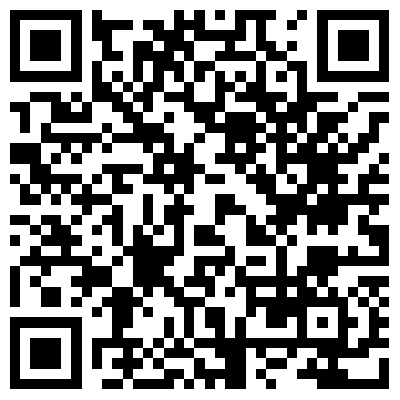
\includegraphics[width=0.4\textwidth]{papers/reedsolomon/images/qrcode_h}
	}
	\subfigure[]{
	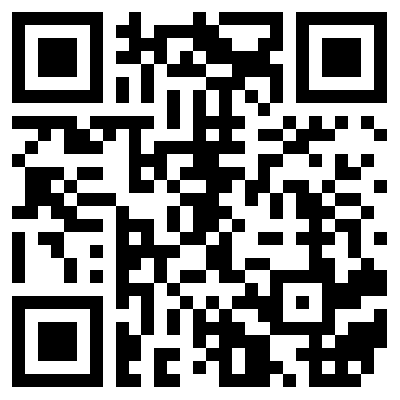
\includegraphics[width=0.4\textwidth]{papers/reedsolomon/images/qrcode_l}
	}
%	\subfigure[]{
%	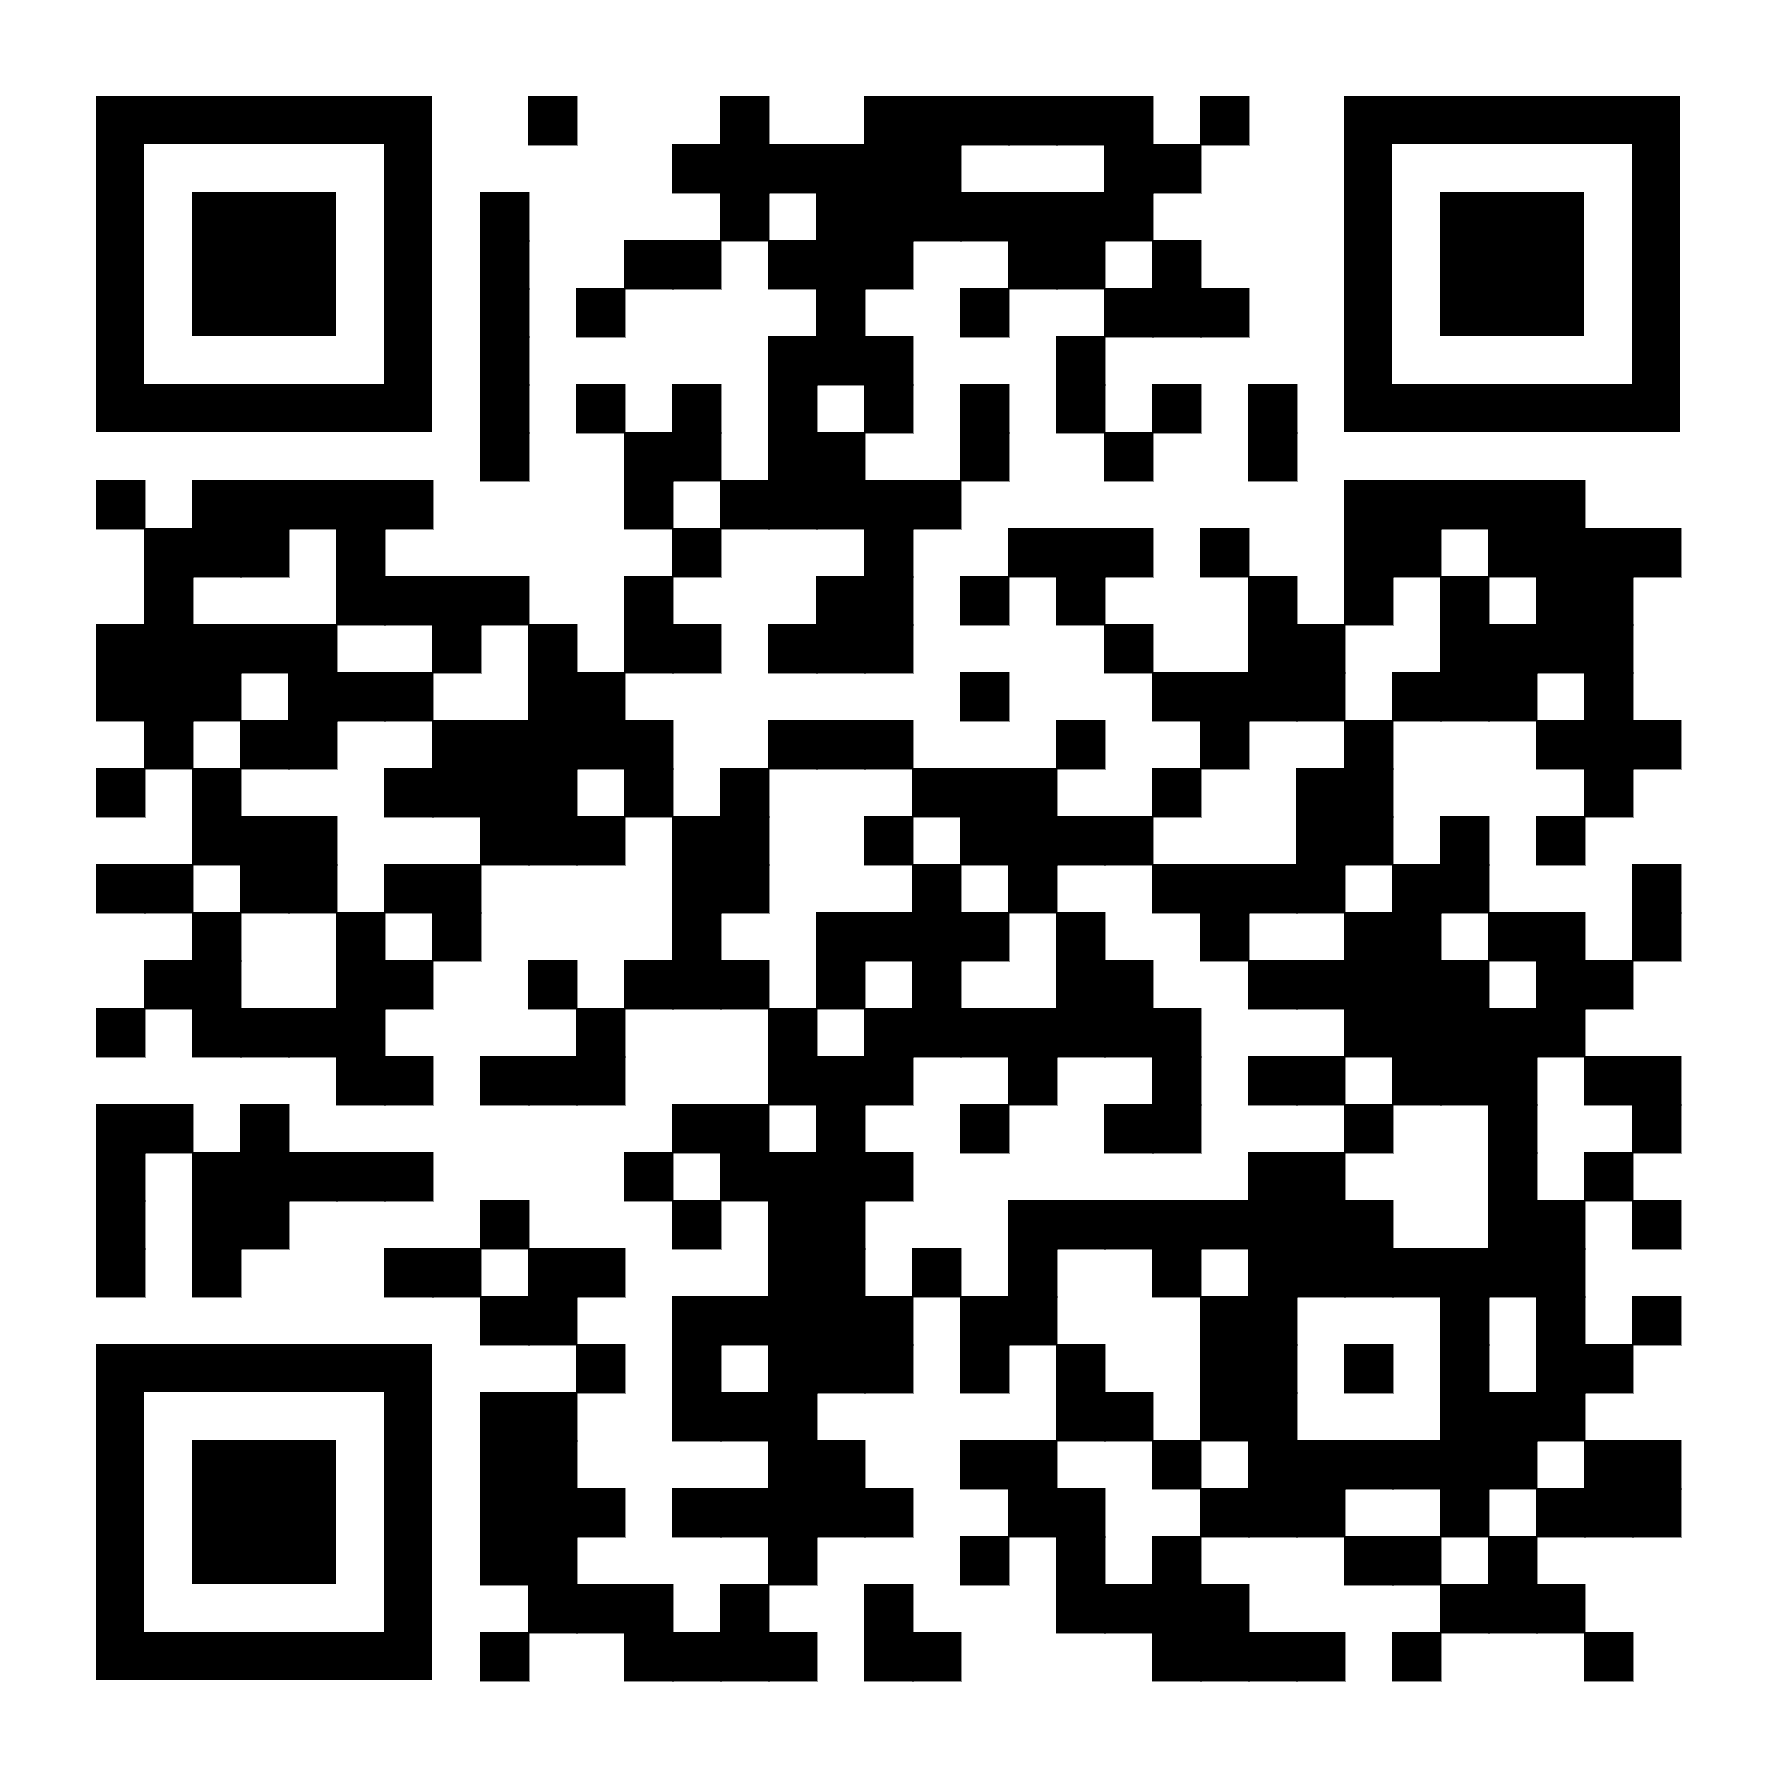
\includegraphics[width=0.4\textwidth]{papers/reedsolomon/images/designer_qrcode_ohnelogo}
%	}
%	\subfigure[]{
%	
\includegraphics[width=0.4\textwidth]{papers/reedsolomon/images/designer_qrcode}
%	}
	\caption{Anhand der grösse würde man darauf schliessen, dass bei (a) mehr Informationen codiert sind als bei (b). Tatsächlich aber beinhalten beide Codes die gleiche Information. Das liegt daran, da die Fehlerkorrekturfähigkeit von QR-Codes sich in insgesamt vier Levels aufteilen lassen. Der höchste Fehlerkorrektur-Level, der bei (a) angewendet wurde, ist in der Lage, bis zu 30\% der Daten wiederherzustellen. Der kleinste Level schafft etwa 7\%, der in (b) veranschaulicht wird. Da die Grösse also nichts über die Menge an Daten aussagt, könnte es sich bei (a) auch um einen Code mit viel Nutzdaten und kleinem Fehlerkorrektur-Level handeln. Der Unterschied ist von Auge nicht sichtbar.}
	\label{fig:qr}
\end{figure}

\begin{figure}
	\centering
%	\subfigure[]{
%		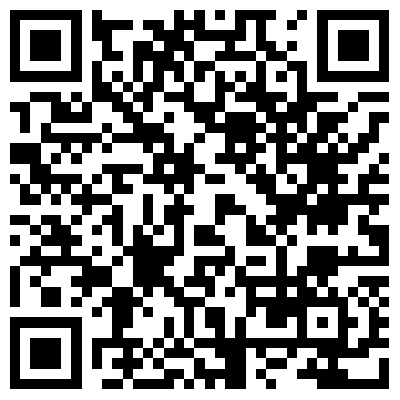
\includegraphics[width=0.4\textwidth]{papers/reedsolomon/images/qrcode_h}
%	}
%	\subfigure[]{
%		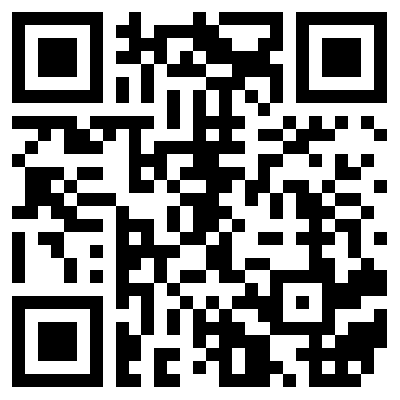
\includegraphics[width=0.4\textwidth]{papers/reedsolomon/images/qrcode_l}
%	}
	\subfigure[]{
		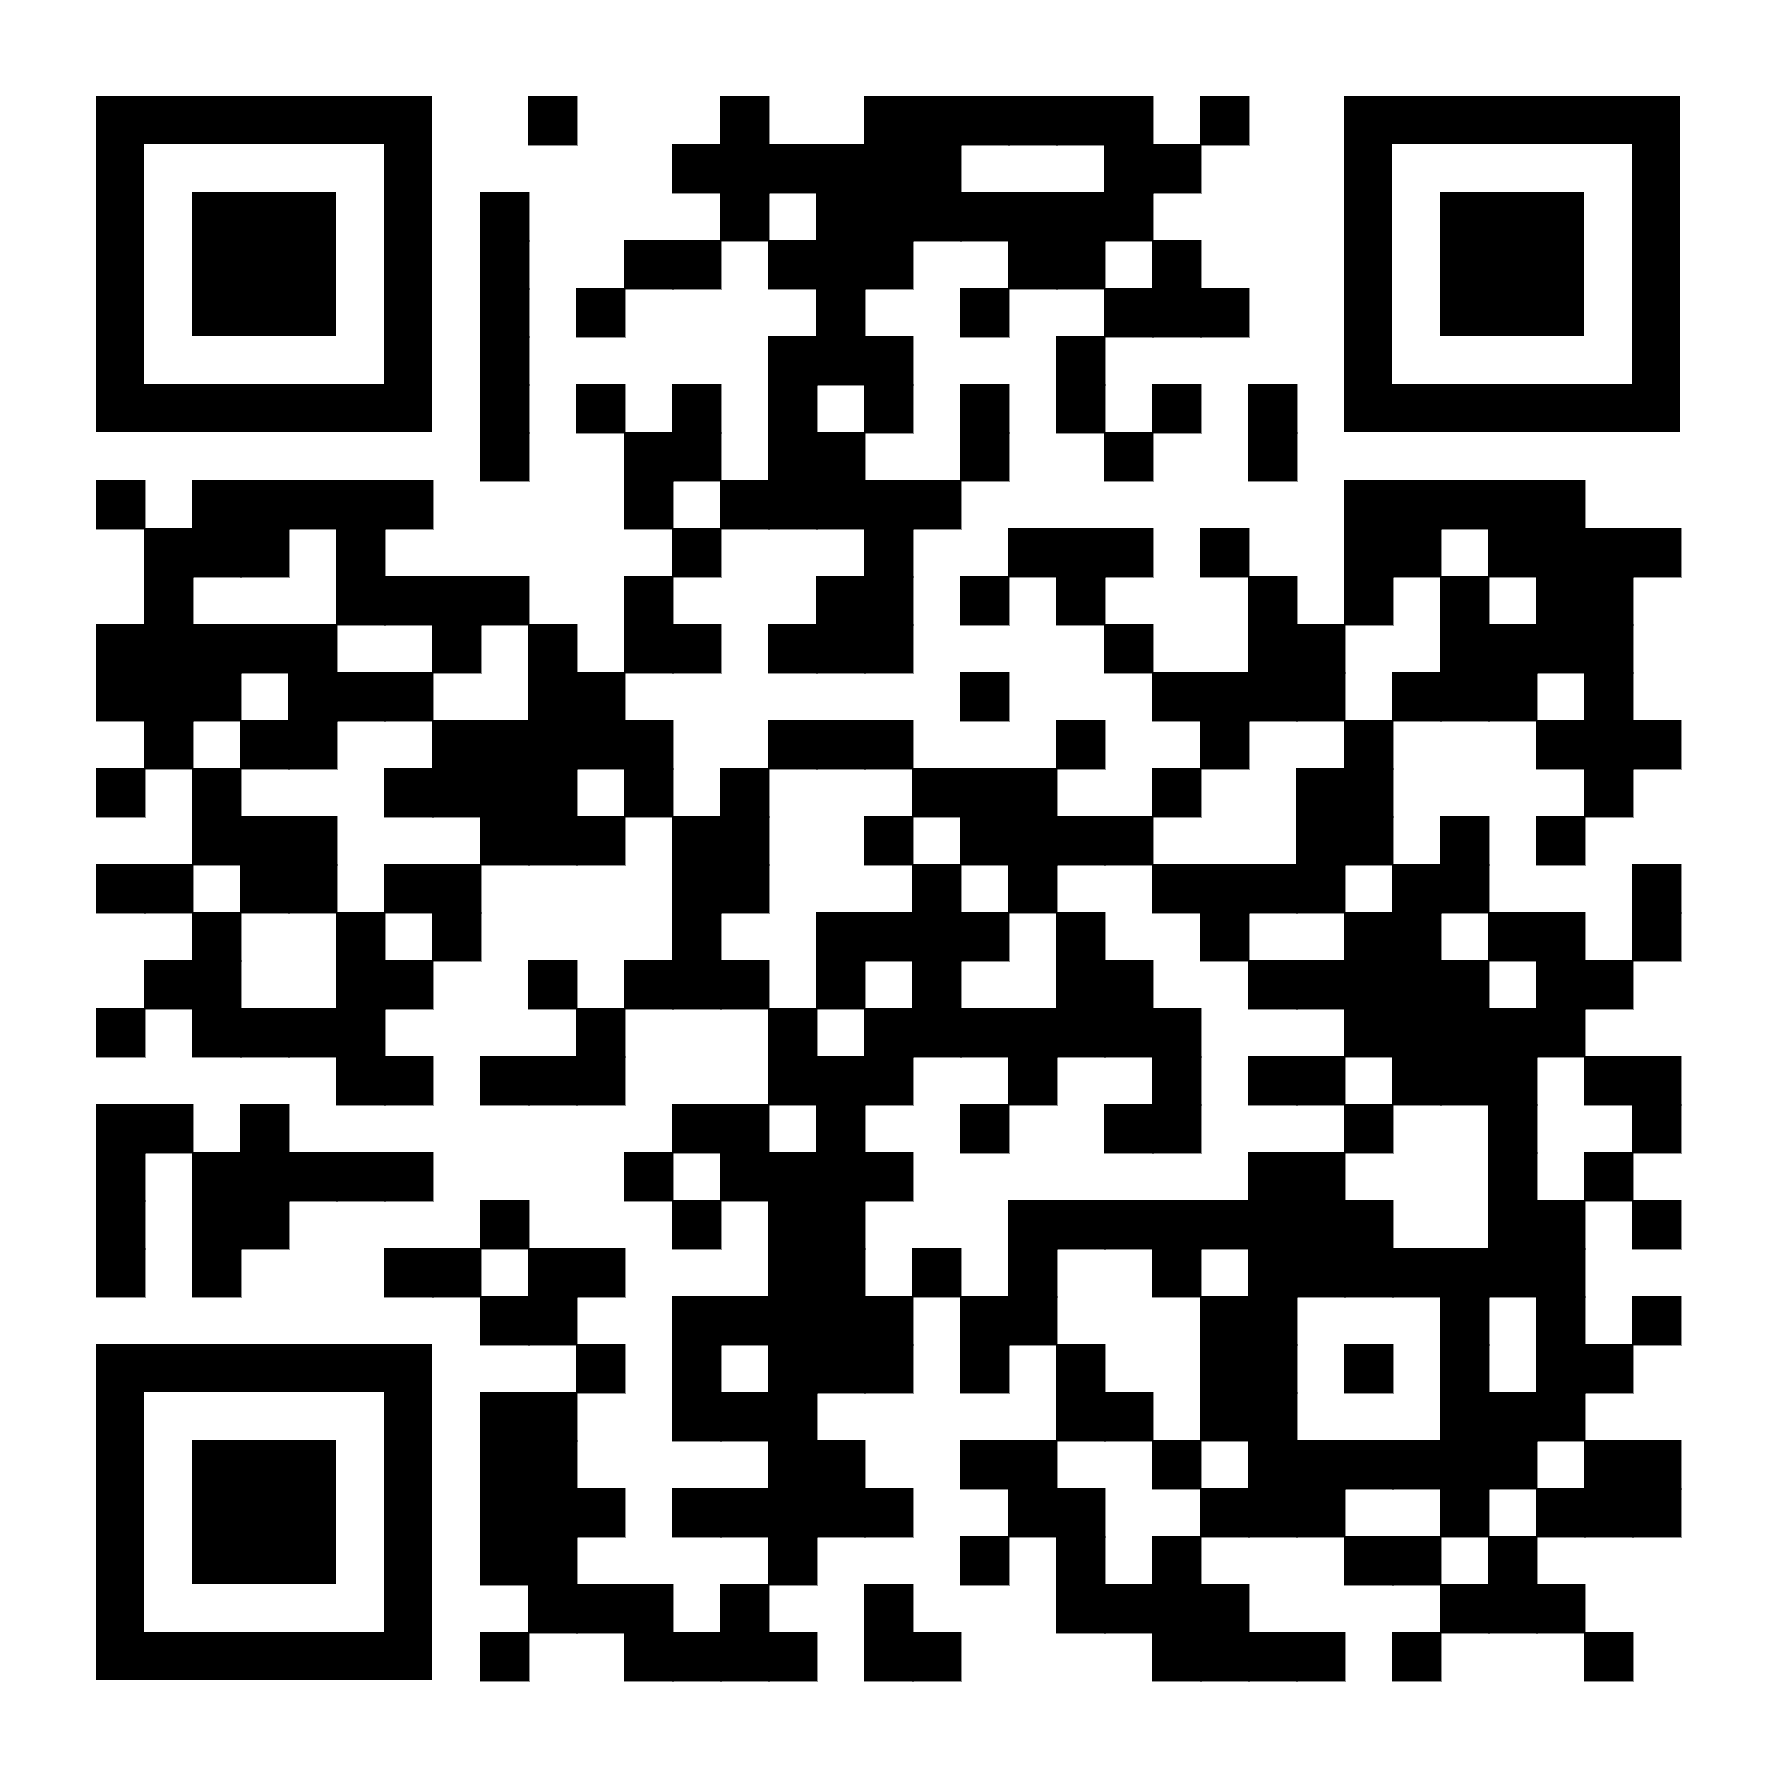
\includegraphics[width=0.4\textwidth]{papers/reedsolomon/images/designer_qrcode_ohnelogo}
	}
	\subfigure[]{
		
\includegraphics[width=0.4\textwidth]{papers/reedsolomon/images/designer_qrcode}
	}
	\caption{Während (a) noch einen unveränderten QR-Code repräsentiert, handelt es sich bei (b) nun um einen Designer-QR-Code. Beide Codes verfügen über einen mittleren Fehlerkorrektur-Level von theoretisch 15\%. Da bei (b) jetzt einen Teil des Codes durch ein Logo verdeckt wird, schränkt sich die Fehlerkorrekturfähigkeit je nach Grösse des verdeckten Teils mehr oder weniger stark ein. Unser Designer-Code in (b) ist nur noch in der Lage etwa 9\% des Codes zu rekonstruieren.}
	\label{fig:designqr}
\end{figure}

\subsection{QR-Codes}
\index{QR-Code}%
Quick Response Codes oder auch QR-Codes funktionieren nach einem sehr ähnlichen Prinzip wie in unserem Beispiel der Abschnitte \ref{reedsolomon:section:codebsp} - \ref{reedsolomon:section:rekonstruktion} nur das QR-Codes in einem $\mathbb{F}_{256}$ Körper arbeiten.
Die physische Grösse eines Codes ist stark abhängig von der Menge an codierten Daten sowie dem verwendeten Fehlerkorrektur-Level.
Es ist so auf dem ersten Blick nicht ersichtlich, wie viel Nutzinformationen ein QR-Code enthält.
Die QR-Codes in Abbildung \ref{fig:qr} zeigen jeweils die gleiche Information mit unterschiedlichem Fehlerkorrektur-Level.
Codes mit einem höheren Korrektur-Level können auch für Designer-Codes zweckentfremdet werden.
\index{Designed-QR-Code}%
Dabei wird z.~B.~das Firmenlogo oder einen Schriftzug über den QR-Code gelegt, ohne das die Funktion des Codes beeinträchtigt wird. Ein Beispiel dazu ist in Abbildung \ref{fig:designqr} zu finden. 

% 

%So kann auf den ersten Blick nicht 
%
%
% funktionieren nach einem sehr ähnlichen Prinzip wie in unserem Beispiel, nur dass QR-Codes in einem $\mathbb{F}_{256}$ Körper arbeiten. Je nach grösse der Codierung ist der QR-Code im Endeffekt robuster gegen Beschädigungen. Bei Low Level Codes können 7\% der Daten Wiederhergestellt werden, beim High Level Code sind das sogar 30\%. 

